\section{Adresstransformation}

\textbf{Logischer Cache}: Cache über logische Adressen ansprechen. Adresstransformation erfolgt nach dem Cache.

\textbf{Physischer Cache}: Cache über physische Adressen ansprechen. Adresstransformation erfolgt vor dem Cache.


Zwei Ansätze:

\textbf{Page-Transformation}: Aufteilen des physischen Speichers in Seiten (Pages) einheitlicher Grösse.

\textbf{Segment-Transformation} (Segmentierung): Aufteilen des physischen Speichers in Bereiche (Segments) flexibler Grösse (Grösse von OS bestimmt).

\subsection{Einstufige Page-Transformation}

Pages haben eine feste Länge von $2^k$ Byte.
Die relative Adresse innerhalb einer Page ab Seitenanfang wird \textit{Page-Offset} genannt.
Zuordnung von logischen auf physische Pages erfolgt via \textit{Page-Descriptor-Tables} (Umsetzungstabellen) in der MMU.

{\scriptsize
$n$: Anazahl Bit der physischen Adresse\\
$m$: Anazahl Bit der logischen Adresse\\
$k$: Anazahl Bit des Page-Offsets\\
$x$: LS-Bit der physischen Page-Nummer im Page-Desktiptor\\
$A_p$: Physische Adresse (Speicheradresse)\\
$A_L$: Logische Adresse (Programmadresse, effektive Adresse)\\
$PD$: Umsetztabelle (Einträge sind die Page-Deskrptoren)\\
$PD[i]$: Page Desktiptoren-Nummer $i$ (Eintrag im Index $i$ aus $PD$)\\
|: Aneinanderfügen von Bitmuster (Concatenation)\\
<$i$..$j$>: Bit-Positionen aus einem Bitmuster\\
$+$: Addition von Bitmuster
}

\formula{$A_p$<$n$-1..0> = $PD$[$A_L$ <$m$-1..$k$>]<$x$+($n$-1-$k$)..$x$>|$A_L$<$k$-1..0>}

\begin{center}
    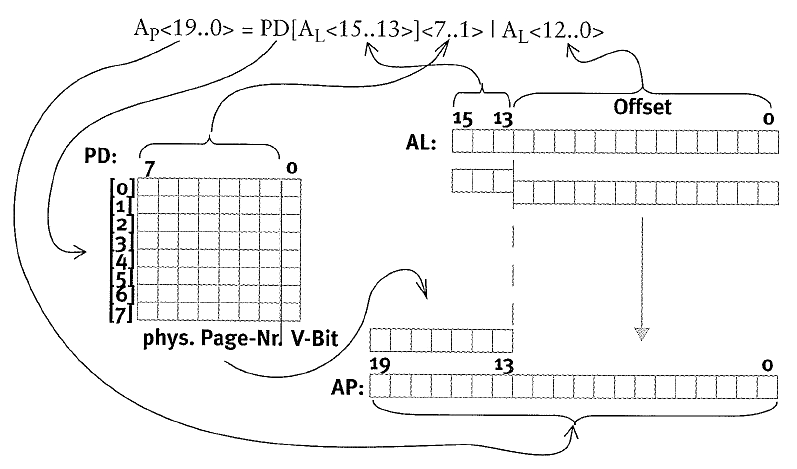
\includegraphics[width=\linewidth]{PageTransformationsformel.png}
    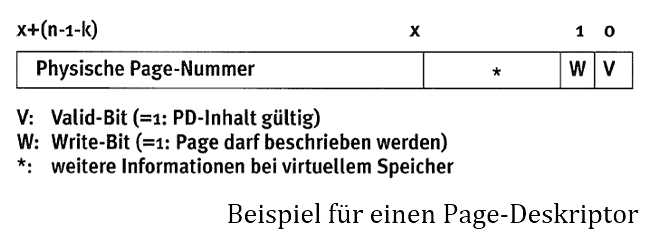
\includegraphics[width=\linewidth]{PageDeskriptor.png}
\end{center}


\subsection{Mehrstufige Page-Transformation}

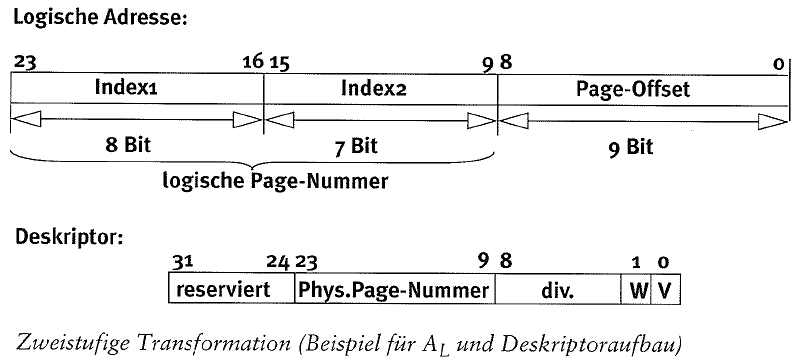
\includegraphics[width=\linewidth]{MehrstufigePagetransformation.png}
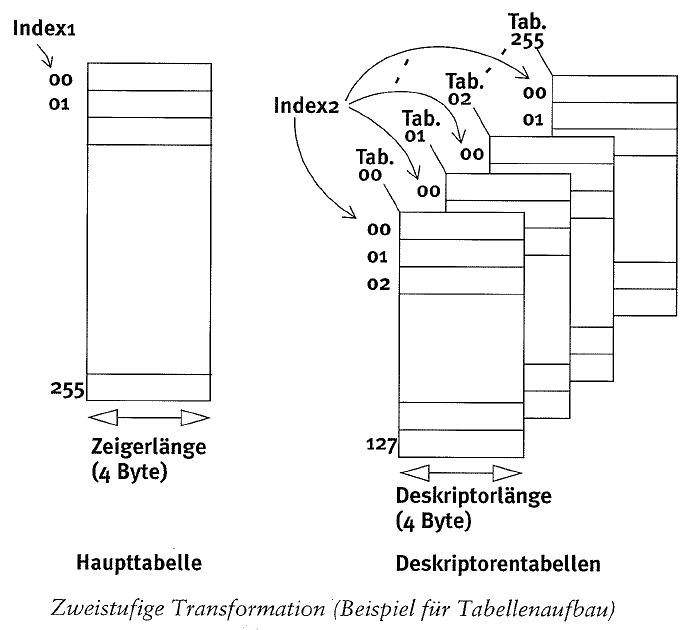
\includegraphics[width=\linewidth]{MehrstufigeTransformation.png}


\section{Virtueller Speicher}

Virtualisierun gerlaubt Ausführung von Programmen, die nicht vollständig in Hauptspeicher geladen sind. Basierend auf Paging.

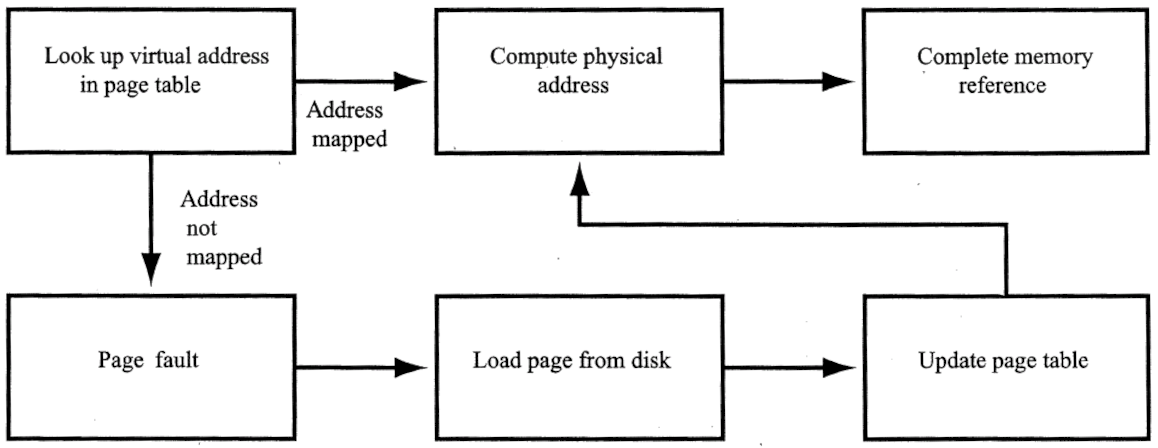
\includegraphics[width=\linewidth]{MMU.png}


\section{Prozessorleistung}

\subsection{Rechenleistung}

\formula{$\mathit{Time} = \dfrac{\mathit{Seconds}}{\mathit{Program}} = \dfrac{\mathit{Instructions}}{\mathit{Program}} \cdot \dfrac{\mathit{Clock cycles}}{Instruction} \cdot \dfrac{\mathit{Seconds}}{\mathit{Clock cycle}}$}

\subsection{Speed-up gemäss Amdahl's Law}

\formula{$T_m = T_s + T_p = \dfrac{s \cdot A}{L_{SISD}} + \dfrac{p \cdot A}{n \cdot L_{SISD}} = \dfrac{A}{L_{SISD}} \cdot (s + \dfrac{p}{n})$}
\formula{$\mathit{Speedup} = \dfrac{L_{MIMD}}{L_{SISD}} = \dfrac{1}{s + \dfrac{1 - s}{n}}$}